\chapter{Experiment and Result}
brief of experiment and result.
\section{Experiment}
Please tell how the experiment conducted from method.

\section{Result}
Please provide the result of experiment

\section{Cokro Edi Prawiro / 1164069}

\subsection{Teori}
\begin{enumerate}
\item Jelaskan apa itu klasifikasi teks, sertakan gambar ilustrasi buatan sendiri.\par
klasifikasi teks adalah cara untuk memilah-milah teks berdasarkan parameter tertentu baik itu jenis teks atau jenis dari dokumen yang terdapat kumpulan teks didalamnya, sedangkan teks itu sndiri merupakan sekumpulan kata yang dapat dibaca. bisa berupa buku, majalah, rambu-rambu dan lain sebagainya. agar lebih jelas dapat dilihat pada gambar \ref{c55}

\item Jelaskan mengapa klasifikasi bunga tidak bisa menggunakan machine learning, sertakan ilustrasi sendiri.\par
Klasifikasi bunga tidakdapat menggunakan mesin learning dikarenakan jenis-jenis bunga banyak yang mirip bahkan banyak bunga yang serupa tetapi tidak sama. oleh karena itu klasifikasi bunga tidakbisa di gunakan oleh mesin learning dikarenakan jika salah satu inputan ciri-ciri dari siatu bunga di inputkan kemungkinan jawaban dari mesin learning itu tidak tepat contoh dimasukan inputan ciri ciri bunga mawar putih kemudian mesin learning menjawab bahwa itu bunga mawar merah. untuk lebih jelasnya dapat dilihat pada gambar \ref{c56}

\item Jelaskan bagaimana teknik pembelajaran mesin pada teks pada kata-kata yang digunakan di youtube,jelaskan arti per atribut data csv dan sertakan ilustrasi buatan sendiri.\par
cara pembelajaran teks yang di gunakan youtube yaitu dengan cara merekam data yang sering di inputkan oleh user pada menu pencarian youtube. sehingga pada saat user akan mencari data yang serupa seringkali youtube menyediakan opsi atau rekomendasi-rekomendasi dari pencaharian. contoh saya menuliskan m maka muncul opsi pilihan master chep dan lainya yang berawalan m rekomendasi yang muncul merupakan kata-kata yang sering di cari oleh banyak user atau sering di buka oleh user itu sendiri untuk lebih jelasnya dapat dilihat pada gambar \ref{c57}

\item Jelaskan apa yang dimaksud vektorisasi data.\par
vektorisasi data merupakan pemechan data menjadi bagian bagian yang lebih sederhana contoh pada satu paragraf terdiri dari 200 kata kemudian dilakukan vektorisasi dengancara membagi-bagi kata dalam paragraf tersebut ke dalam kalimat-kalimat yang terpisah kemudian di pecah lagi menjadi data dalam perkata selanjutnya kata kata tersebut di terjemahkan.

\item Jelaskan apa itu bag of words dengan kata-kata yang sederhana dan ilustrasi sendiri.
 bag of words merupakan peroses penyederhanaan kata-kata yang asalnya tersiri dalam satu kalimat atau satu paragraf di ubah menjadi perkata kemudian kata-kata tersebut di kumpulkan menjadi satu kelompok tanpa ada arti dari kata-kata yang telah di kumpulkan tersebut lalu di hitung frekuensi kemunculan dari kata tersebut. supaya lebih jelas dapat dilihat pada contoh gambar \ref{c58} :

\item Jelaskan apa itu TF-IDF, ilustrasikan dengan gambar sendiri.
 TF-IDF merupakan metode untuk menghitung bobot dari kata yang sering muncul pada suatu kalimat. metode ini menghitung nilai TF atau Term Frequency dan IDF atau Inverse Document Frequency pada setiap kata pada kalimat yang dijadikan acuan kata pada metode ini sering di sebut token adapun rumus dari metode ini dapat dilihat pada gambar \ref{c59} dan untuk hasil ujicobanya dapat di lihat pada gambar \ref{c60} dan gambar \ref{c61}.

\end{enumerate}

\subsection{Praktek Program}

\subsection{Penanganan Error}

\begin{figure}
      \centerline{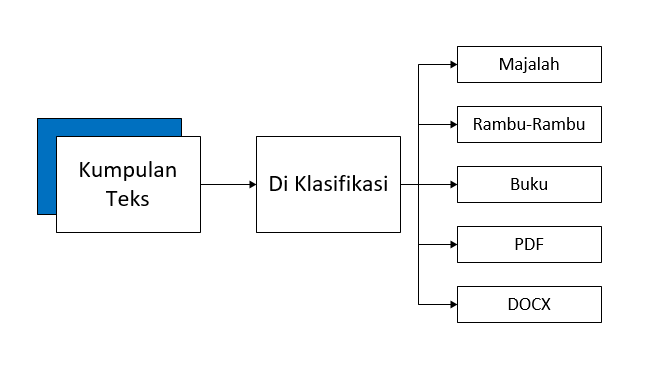
\includegraphics[width=1\textwidth]
      {figures/cokro/c55}}
      \caption{Ilustrasi clasifikasi Teks}
      \label{c55}
      \end{figure}

\begin{figure}
      \centerline{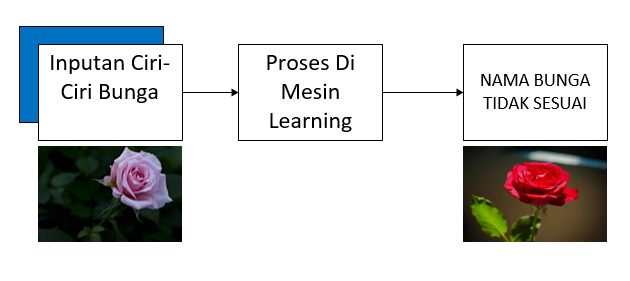
\includegraphics[width=1\textwidth]
      {figures/cokro/c56}}
      \caption{Ilustrasi Bunga Tidak bisa dibaca di Mesin Learning}
      \label{c56}
      \end{figure}

\begin{figure}
      \centerline{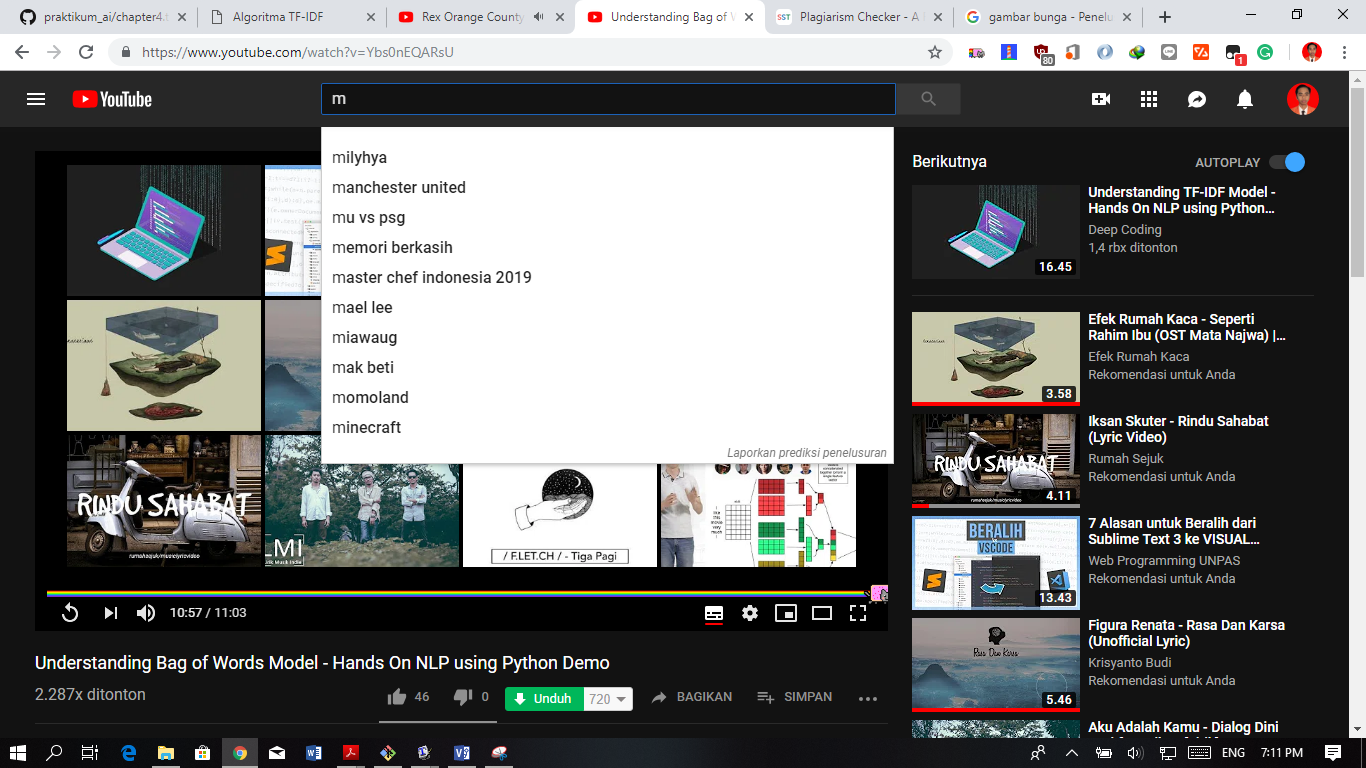
\includegraphics[width=1\textwidth]
      {figures/cokro/c57}}
      \caption{contoh hasil pembelajaran text di youtube}
      \label{c57}
      \end{figure}

\begin{figure}
      \centerline{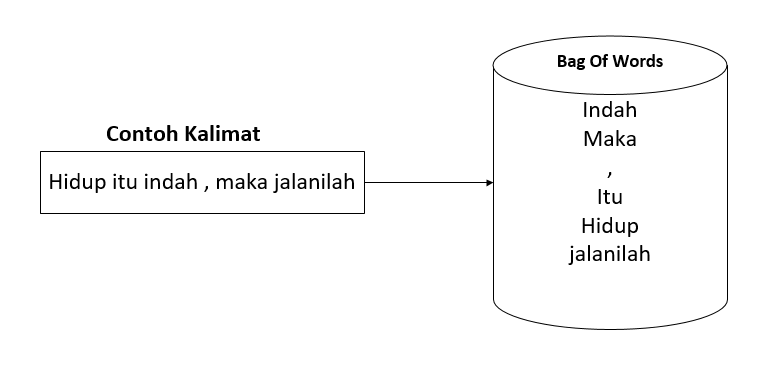
\includegraphics[width=1\textwidth]
      {figures/cokro/c58}}
      \caption{Ilustrasi bag of words}
      \label{c58}
      \end{figure}

\begin{figure}
      \centerline{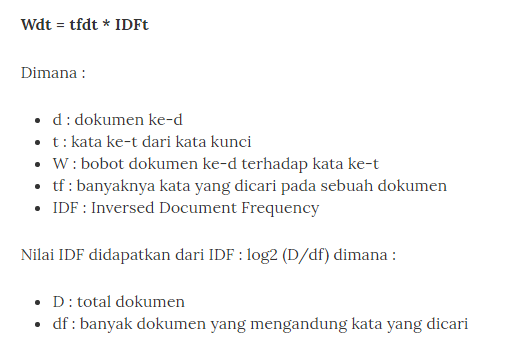
\includegraphics[width=1\textwidth]
      {figures/cokro/c59}}
      \caption{Rumus  TF-IDF}
      \label{c59}
      \end{figure}

\begin{figure}
      \centerline{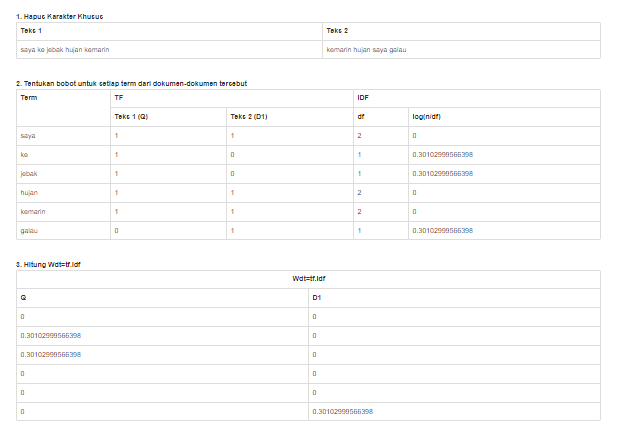
\includegraphics[width=1\textwidth]
      {figures/cokro/c60}}
      \caption{Hasil Perhitungan TF-IDF}
      \label{c60}
      \end{figure}

\begin{figure}
      \centerline{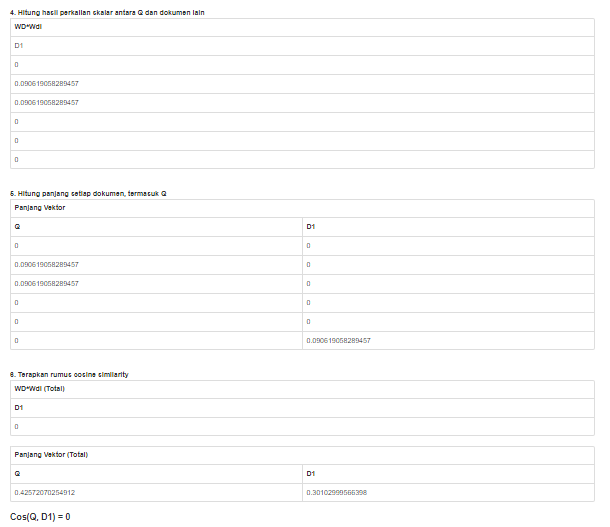
\includegraphics[width=1\textwidth]
      {figures/cokro/c61}}
      \caption{Hasil Perhitungan  TF-IDF}
      \label{c61}
      \end{figure}